\section{Introduction} %\label{sec:extenstion_introduction}

This chapter extends the previous work in \cite{calderon_scalable_2023}. The main new contributions are summarized as follows. First, we introduce a new spatial partitioner, based on the kd-tree partitioning strategy, for constructing overlay  DCELs (section \ref{sec:pstrategies}). Since it better utilizes the data  distributions in optimizing DCEL partitions, it leads to noticeably improved performance. The new partitioning strategy contrasts with the original strategy that employed space-partitioning techniques based on quadtrees. 

Second, we enable overlay DCELs to take scattered and noisy line segments as input instead of being limited to clean polygon data.  This builds on the work on scalable polygonization in \cite{abdelhafeez_ddcel_2023} to enable overlays of real datasets that consist of massive sets of line segments that cannot currently be handled by any existing technique.  

For example, Figure \ref{fig:extension_dcel_example} shows the fundamental components of a DCEL.  In addition, we note a couple of special half-edges. \textit{Dangles} are the half-edges with one or both ends not incident on another half-edge endpoint. Half-edge \textit{$\overrightarrow{fj}$} and its twin are both considered dangle edges.  \textit{Cut-Edges} are the half-edges connected at both ends but do not form part of a polygon. The half-edge \textit{$\overrightarrow{dg}$} and its twin are considered cut-edges.

\begin{figure}
    \centering
    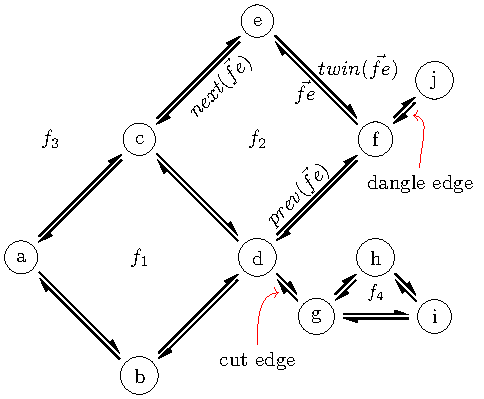
\includegraphics[width=0.6\linewidth]{chapterExtension/dcel_example2}
    \caption{Components of the DCEL structure with dangle and cut edges.}\label{fig:extension_dcel_example}
\end{figure}

The rest of this chapter is organized as follows.  Section \ref{sec:extension_methods} details the polygon extraction process for line input adaptation. It also extends the overlay method by supporting the overlay of dangle and cut edges. In Section \ref{sec:extension_experiments} we also provide additional experiments, to quantify the benefits of the kd-tree based strategy, as well as the performance on the datasets with large volumes of line segments.
